\subsubsection{Database}\label{subsec:databasedesign}

In this framework, a database was needed to keep track of all information related to users and games they are playing. The database is designed with flexibility in mind which means that the logic behind a game is responsible for interpreting the data in the database. \figref{fig:erdiagram} shows the entity relation diagram for the database without attributes. The database is structured as follows:

\begin{figure}[H]
  \centering
  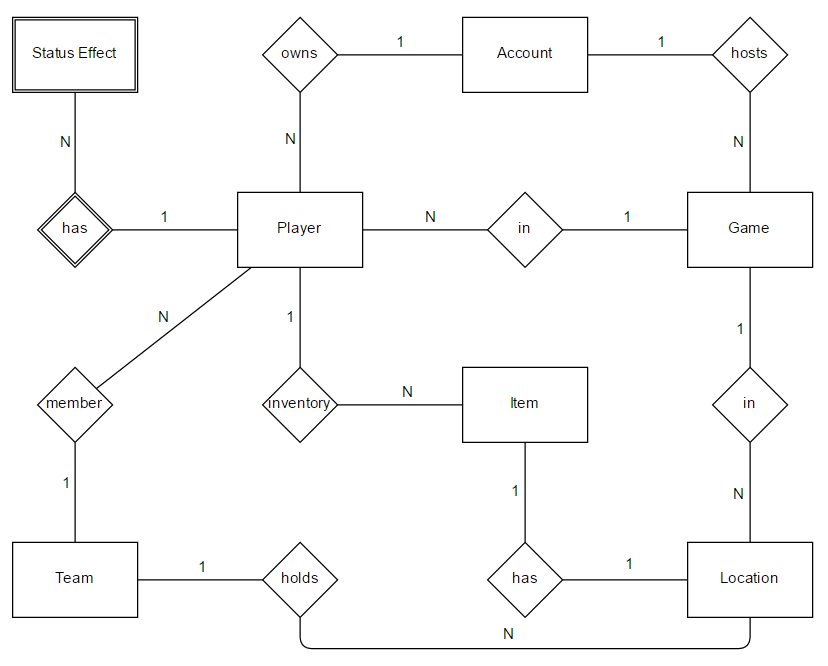
\includegraphics[width=\textwidth]{billeder/serverdiagram.png}  
  \caption{Diagram displaying the server structure}
  \label{fig:erdiagram}
\end{figure}

\paragraph{Account}
The Account entity represent the users in the system. An account can host games represented by the host relation and take part in games represented as owning a player in a particular game.

\paragraph{Player}
This entity represents a user playing in a game. A player can hold items, have status effects and be a member of a team represented by Inventory, has(Status Effect) and Team(is\_member) respectively. The player entity also contains score and location etc. for a particular player in a game.

\paragraph{Game}
This entity represent games either \textit{starting up}, \textit{in progress} or \textit{ended}.

\paragraph{Status Effect}
Effects on a player is represented by this entity. An effect could be \textit{disabled until time} on a particular player. Status Effects have an effect type which the game logic is responsible for defining.

\paragraph{Team}
Players can be members of teams in a game, though a player is not required to be on a team to allow free for all game modes.

\paragraph{Item}
Items represent any object in the inventory of players or on a location in the game world. Items can be anything from objects players can "pick up" to a capture-able area in the game world. The attributes and behavior of items are defined by game logic.

\paragraph{Location}
A location is an item in the game world that can belong to a team. To own a location, a team must take it first.



